% !TEX TS-program = lualatex
% !TEX encoding = UTF-8 Unicode

\documentclass[]{einformatica}
\usepackage{graphicx}
\usepackage{soul}
\usepackage{booktabs}
\usepackage{hyphenat}
\usepackage[all]{nowidow}
\usepackage{tabularx}
\usepackage{floatrow}
\floatsetup[table]{style=plain,capposition=top}
\renewcommand\topfraction{.95}
\renewcommand{\textfraction}{0.05}
\usepackage{refcount} 
\usepackage[noadjust]{cite}

\usepackage{xcolor}
\usepackage{hyperref}
\hypersetup{
    urlbordercolor = black,
    pdfborderstyle={/S/U/W 1},
}

\usepackage{cleveref}
\usepackage{amsmath}
\usepackage{amssymb}

% Please, add only really required packages here

\begin{document}

\title{Text-to-SQL Dataset Quality Assessment: The First Open-Source Validation Framework}

\shortauthorshead{Sabadosh}

\eIsubmitted{1 Nov. 2024} 
\eIrevised{15 Jan. 2025} 
\eIaccepted{20 Feb. 2025}
\eIpublished{1 Mar. 2025} 

\EIauthorI
   {Volodymyr}
   {Sabadosh}
   {Your Institution, Your Country}
   {your.email@institution.edu}
   {0000-0000-0000-0000} % Replace with your ORCiD ID
   {*} %  if star present means corresponding author

% Add additional authors if needed using \EIauthorII, \EIauthorIII, etc.
 
\keywordset{Text-to-SQL system, dataset quality, LLM, SQL validation, semantic evaluation, empirical software engineering} 

\begin{abstract}[en]
\textbf{Context}: 
Text-to-SQL systems that translate natural-language questions into SQL have advanced rapidly with large language models (LLMs). However, progress depends critically on the quality of benchmark datasets used for training and evaluation. \\
\textbf{Objective}: 
Our objective is to develop and demonstrate a comprehensive automated system for evaluating Text-to-SQL dataset quality through multi-level validation addressing current gaps in systematic quality assessment. \\
\textbf{Method}: 
We introduce a Text-to-SQL dataset analysis tool, built on a streaming, protocol-oriented, dependency-injected architecture with pluggable analyzers. Our most novel component is the semantic correctness evaluator using multi-model LLM consensus voting. We validate the framework by conducting a complete audit of all 11,840 examples in the Spider 1.0 benchmark across its three partitions (test, dev, train). \\
\textbf{Results}: 
Applying the framework to all 11,840 examples of the Spider 1.0 benchmark, we obtain 100\% parsability and 99.97\% executability of SQL queries. Despite this, schema analysis reveals 89 invalid foreign keys, 40,673 referential integrity violations concentrated in two databases, and systematic quality differences across partitions. LLM-based semantic validation identifies that only 60--70\% of examples receive high-confidence correct verdicts, with 18--26\% exhibiting model disagreement. \\
\textbf{Conclusions}: 
Multi-layer automated validation exposes hidden weaknesses in Text-to-SQL benchmarks that are invisible to standard exact-match or execution-based metrics. We release the first open-source comprehensive validation framework to enable systematic quality assessment of existing and future Text-to-SQL datasets.
\end{abstract}

\maketitle 

\section{Introduction}\label{sec:Introduction}

Text-to-SQL systems, which transform natural language queries into structured SQL queries, are experiencing a period of rapid development driven primarily by remarkable progress in Large Language Models (LLMs). The task has evolved from a specialized research challenge into a practical technology deployed across major cloud platforms and data analytics tools.

From a scientific perspective, the Text-to-SQL task serves as an important test of LLMs' capacity for structured reasoning and simultaneous understanding of natural language semantics and formal programming language syntax, making it a valuable benchmark for assessing the limits and capabilities of contemporary language models.

\begin{figure}[htbp]
  \centering
  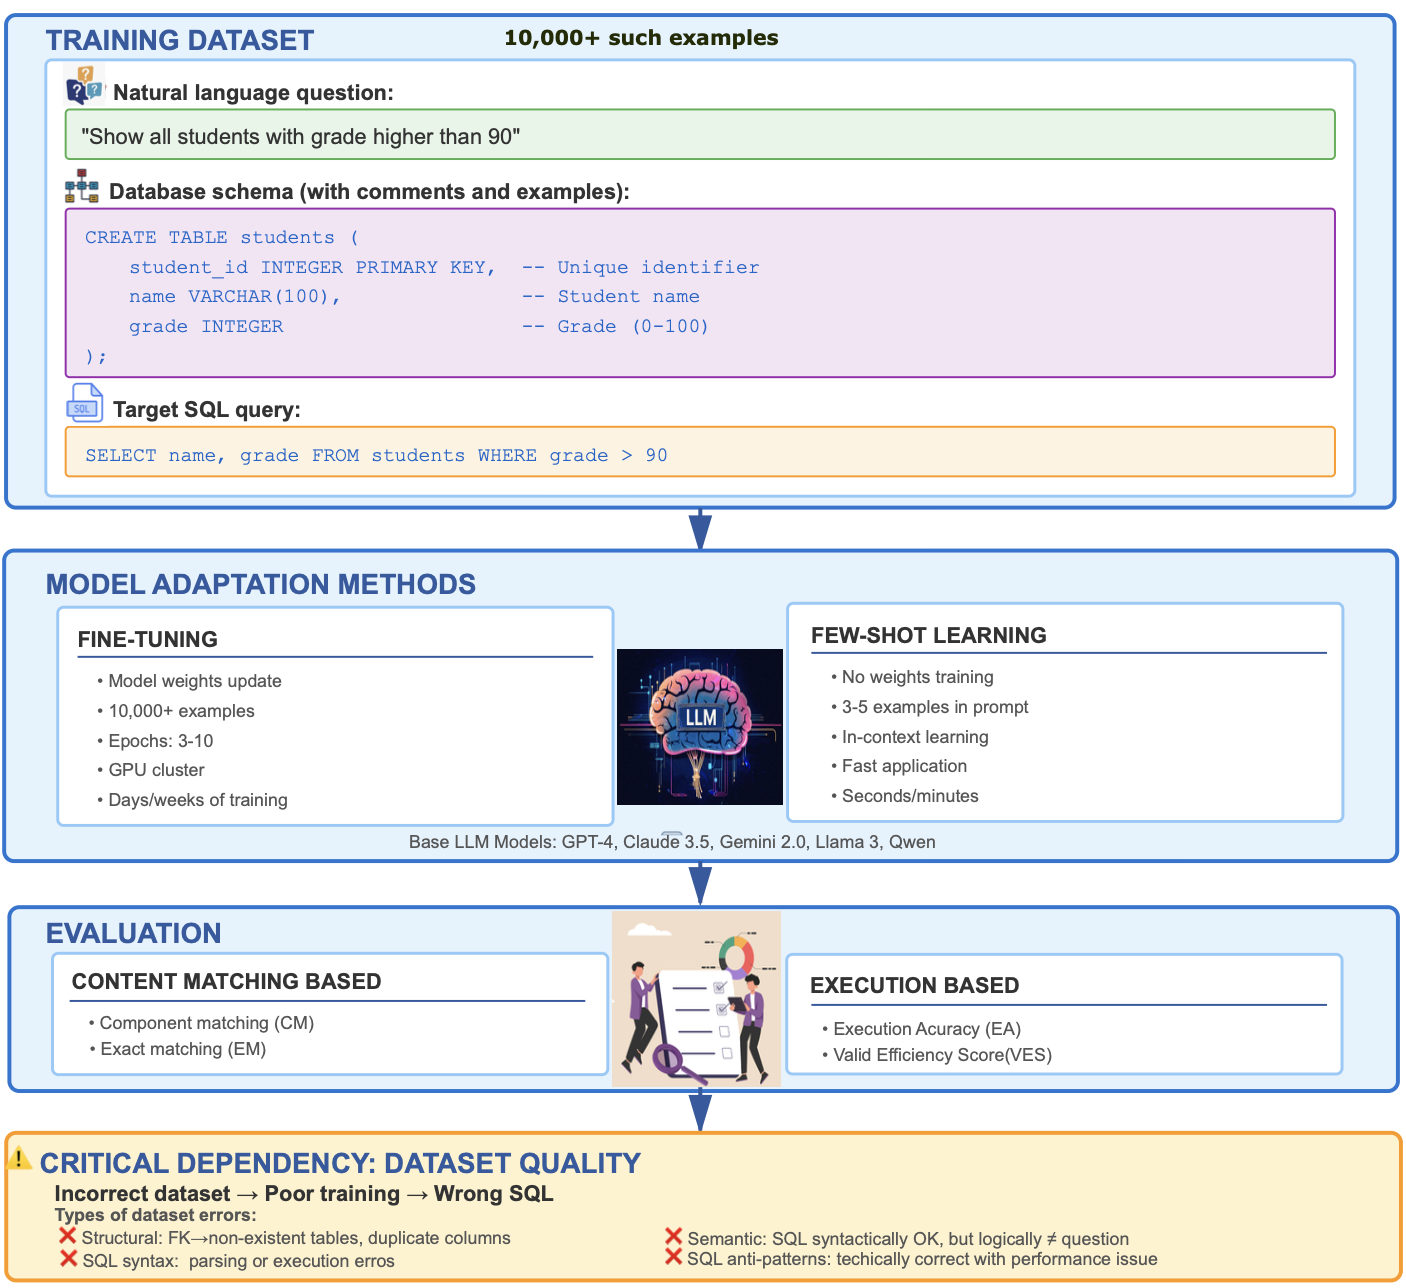
\includegraphics[width=0.8\textwidth]{figures/fig1_training_process.png}
  \caption{Complete training pipeline for LLMs in Text-to-SQL systems}
  \label{fig:training_process}
\end{figure}

From a practical standpoint, Text-to-SQL LLM systems are being actively deployed by leading cloud platforms. Snowflake Copilot can generate SQL from natural language in Snowsight~\cite{snowflake_copilot}; Databricks AI/BI Assistant brings conversational data exploration to Azure environments~\cite{databricks_genie}; Microsoft Fabric integrates Copilot directly into SQL database workloads~\cite{microsoft_fabric_copilot}.

The typical process of training LLMs for Text-to-SQL tasks includes three key components (Figure~\ref{fig:training_process}): a training dataset containing triplets of \{natural language question, database schema, Target SQL query\}, a supervised fine-tuning step, and evaluation on a held-out test set. The entire pipeline's effectiveness hinges fundamentally on dataset quality, as errors and inconsistencies propagate directly into model behavior.

Despite the central role of datasets, most work on Text-to-SQL focuses on model architectures, prompting techniques and decoding strategies. The quality of popular benchmarks is typically assumed rather than systematically validated, which creates several critical risks. Dataset errors can manifest as:

\begin{itemize}
\item \textbf{Database schema structural errors}: incorrect foreign keys (references to non-existent tables/columns), duplicate columns, multiple primary keys, unknown data types.
\item \textbf{SQL syntax errors}: queries that cannot be parsed or executed on corresponding databases.
\item \textbf{Semantic mismatches}: SQL queries that are syntactically correct but logically do not correspond to the natural language question (e.g., using SUM instead of AVG, incorrect JOIN conditions, missing necessary filters).
\item \textbf{SQL anti-patterns}: technically correct queries with performance or style issues (SELECT *, absence of LIMIT, functions in WHERE that block index usage).
\end{itemize}

\subsection*{Problem statement}

Therefore, our central research questions are:

\begin{itemize}
\item \textbf{RQ1}: How can we systematically assess the overall quality of Text-to-SQL datasets?
\item \textbf{RQ2}: How accurate and internally consistent are popular Text-to-SQL benchmarks that serve simultaneously as training and evaluation data?
\end{itemize}

\subsection*{Research objective}

This paper addresses these questions by proposing a comprehensive validation framework for Text-to-SQL datasets and using Spider 1.0 as the primary end-to-end testbed for the framework. Our work is positioned at the intersection of empirical software engineering, data quality assessment, and natural language processing.

\subsection*{Contribution statement}

The main contributions of this paper are:

\begin{enumerate}
\item A novel multi-layer validation architecture for Text-to-SQL datasets integrating schema validation, syntax analysis, execution testing, antipattern detection, and LLM-based semantic verification.
\item The first comprehensive empirical audit of all three Spider 1.0 partitions (11,840 examples total) across five complementary quality dimensions.
\item An open-source implementation of the validation framework, publicly available to enable reproducible quality assessment of existing and future Text-to-SQL benchmarks.
\item Concrete empirical evidence that widely-used benchmarks contain significant quality issues invisible to standard evaluation metrics.
\end{enumerate}

\subsection*{How the paper is structured}

The rest of this paper is structured as follows: in~\Cref{sec:RelatedWork}, we briefly discuss work done in similar areas by other researchers; in~\Cref{sec:Methods}, we describe the architectural design and implementation of our validation framework; in~\Cref{sec:Results}, we report the results of applying the framework to Spider 1.0. Then, in~\Cref{sec:Discussion}, we discuss the collected results and threats to validity, and we conclude the paper in~\Cref{sec:Conclusions}.

\section{Related Work}\label{sec:RelatedWork}

\subsection{Text-to-SQL Benchmarks and Datasets}

The development of Text-to-SQL systems has been fundamentally shaped by the evolution of benchmark datasets. Early large-scale efforts, particularly WikiSQL~\cite{zhong2017seq2sql}, provided a foundational testbed with 80,654 examples but limited complexity (single-table queries only).

The release of Spider~\cite{yu2018spider} at EMNLP 2018 marked a pivotal advancement in the field. Spider comprises 10,181 natural-language questions mapped to 5,693 unique SQL queries across 200 databases spanning 138 domains. Its structural complexity (multi-table joins, nested queries, set operations) and cross-domain design (disjoint training and test databases) established it as the de facto standard for evaluating generalization capabilities.

Complementary benchmarks have emerged to address specific evaluation dimensions not fully captured by Spider. The BIRD benchmark~\cite{bird_benchmark} targets large-scale, content-rich databases (approximately 33 GB total) with extensive schemas (average 27.8 tables per database) to test real-world scalability. CHASE addresses domain-specific challenges through 6,500+ domain-specific examples across healthcare, finance and e-commerce.

Synthetic data generation has emerged as a scalable approach to augment training corpora. Gretel's synthetic Text-to-SQL dataset~\cite{gretel_synth} (Gretel-Synth) offers over 100,000 high-quality examples spanning 100+ distinct domains. OmniSQL~\cite{omnisql} synthesizes data using frontier LLMs with human-in-the-loop validation.

Despite the proliferation of alternative resources, Spider 1.0 remains the most comprehensive and widely adopted benchmark due to its unique combination of scale, structural diversity, annotation reliability, and established research community consensus.

\subsection{Data Quality and Robustness in Text-to-SQL}

Empirical evidence increasingly demonstrates that the quality of training and evaluation data has a direct and often nonlinear influence on the performance of Large Language Models (LLMs) in Text-to-SQL tasks.

The Dr.Spider study~\cite{drspider} provides one of the most rigorous analyses of this phenomenon. By applying controlled perturbations to questions, database schemas, and SQL queries, the authors showed that LLM-based Text-to-SQL systems exhibit substantial brittleness: seemingly minor variations (synonymous phrasing, column reordering, schema aliasing) trigger disproportionate performance degradation.

Complementary findings come from Snowflake's Arctic-Text2SQL study~\cite{arctic_text2sql}, which evaluated the effects of mixing high-quality benchmark data (Spider, BIRD) with various forms of synthetic data, including Gretel-Synth. Results confirmed that data quality matters more than volume: adding low-quality synthetic examples degraded performance despite increased training set size.

\subsection{Dataset Quality Assessment Frameworks}

Although dataset quality is critical for Text-to-SQL system performance, systematic validation methodologies remain limited. A recent contribution addressing this gap is the benchmark analysis framework by Mitsopoulou and Koutrika~\cite{mitsopoulou2025analysis}, which provides statistical characterization of Text-to-SQL datasets through distributional analysis of query complexity, database schema characteristics, and structural features.

However, this analysis remains descriptive rather than diagnostic: it does not assess whether dataset entries are correct or semantically faithful. Several important aspects of dataset quality therefore remain unaddressed: schema validity (foreign key consistency, type compatibility), query correctness (syntax errors, executability), and semantic alignment (whether SQL accurately answers the natural language question).

A complementary perspective is offered by Pandey et al.~\cite{pandey2024ensuring}, who propose a ``data accuracy'' validation framework for enterprise Text-to-SQL systems. Their approach focuses on runtime validation of generated SQL against business rules and expected output patterns but does not address systematic benchmark-scale quality assessment.

Taken together, existing approaches provide important analytical foundations and illustrate the need for quality control, but they do not offer a comprehensive, automated, and scalable solution for validating Text-to-SQL datasets across multiple quality dimensions simultaneously.

\section{Methods}\label{sec:Methods}

\subsection{Architectural overview of the text2sql-dataset-analyzer framework}

In this section we present \texttt{text2sql-dataset-analyzer}, a novel framework and, to the best of our knowledge, the first dedicated tool for systematic, multi-layer quality assessment of Text-to-SQL benchmarks.

\textbf{Design principles.} The system represents a streaming data-processing architecture designed to address the challenges of large-scale Text-to-SQL dataset validation and quality assessment. The architecture prioritizes three core principles: streaming processing to enable analysis of arbitrarily large datasets without loading entire datasets into memory; protocol-oriented design using Python typing.Protocol to establish clear component contracts while maintaining implementation flexibility; and dependency injection to facilitate testing, configurability, and extensibility.

\textbf{Technology Stack.} The implementation relies on a carefully selected technology stack centered on Python 3.11~\cite{python311}, chosen for its mature ecosystem of SQL tooling and support for large language model integration. Core dependencies include DuckDB~\cite{duckdb} for high-performance analytical queries over validation metrics, SQLAlchemy 2.0~\cite{sqlalchemy} for database abstraction and connection pooling, SQLGlot~\cite{sqlglot} for SQL parsing and dialect translation, and \texttt{dependency\_injector}~\cite{dependency_injector} for automated dependency management. YAML configuration via PyYAML~\cite{pyyaml} enables declarative specification of pipeline behavior, including analyzer selection, LLM provider settings, and output formats.

\textbf{User Interface.} User interaction with the system occurs primarily through a command-line interface exposed via the \texttt{text2sql} entry point. The interface supports two distinct operational modes corresponding to the primary use cases: analysis mode for dataset validation and report mode for generating human-readable summaries from previously collected metrics.

\subsection{Five-Layer System Architecture}

The system architecture follows a layered design pattern comprising five distinct layers, each responsible for a specific aspect of the data processing pipeline (Figure~\ref{fig:architecture}). This layered organization promotes separation of concerns, testability, and independent evolution of components.

\begin{figure}[htbp]
  \centering
  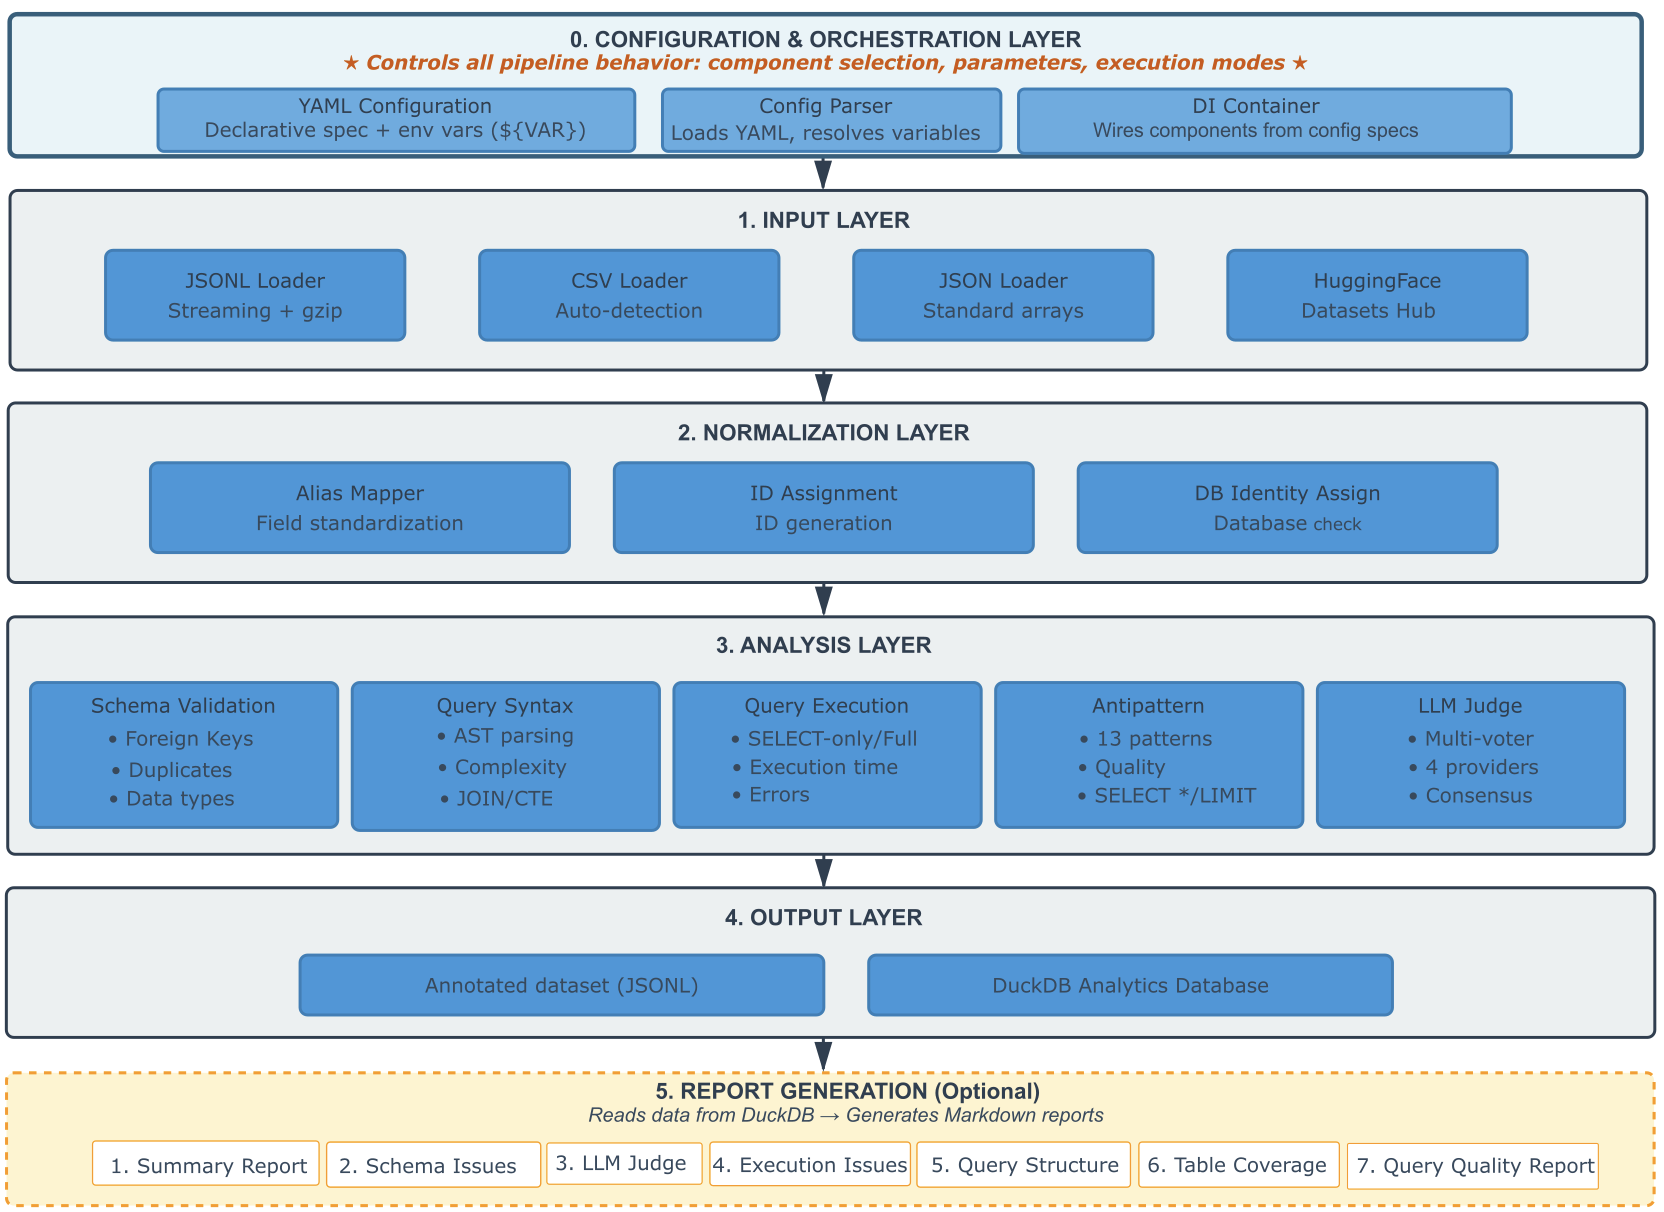
\includegraphics[width=0.9\textwidth]{figures/fig2_architecture.png}
  \caption{Five-layer architecture of the text2sql-pipeline system}
  \label{fig:architecture}
\end{figure}

\textbf{Input Layer.} The Input Layer abstracts heterogeneous data sources behind a common iterator interface. It implements four specialized loaders tailored to data formats prevalent in Text-to-SQL research: SpiderLoader for the Spider benchmark's JSON format, JSONLLoader for line-delimited JSON files produced by synthetic generation pipelines, CSVLoader for tabular exports, and DuckDBLoader for querying previously collected validation results.

\textbf{Normalization Layer.} The Normalization Layer standardizes records originating from diverse datasets through three sequential normalizers. The Alias Mapper reconciles different field names (e.g., \texttt{query} vs \texttt{sql}). The Field Enricher fills missing metadata such as dataset identifiers and difficulty labels. The Database Identity Normalizer (Section~\ref{sec:dbidentity}) ensures every record can be associated with a valid database instance.

\textbf{Analysis Layer.} The Analysis Layer is the computational core, hosting five analyzers that cover complementary quality dimensions of Text-to-SQL data:

\begin{enumerate}
\item \textbf{Schema Validation Analyzer} checks database integrity, including several classes of foreign-key violations, case-insensitive column name duplicates, and type compatibility with the target SQL dialect. It produces per-database validation reports identifying all detected issues with precise location information.

\item \textbf{Query Syntax Analyzer} performs static analysis using the sqlglot parser. It builds abstract syntax trees, derives normalized complexity scores on a 0--100 scale based on SQL constructs and nesting depth, counts structural features (JOINs, subqueries, aggregations), and classifies difficulty into five levels (Easy, Medium, Hard, Extra Hard, Expert).

\item \textbf{Query Execution Analyzer} evaluates dynamic executability within the corresponding database. Queries are run in a sandboxed, SELECT-only mode; execution time and row counts are recorded, and failures are logged with detailed error messages.

\item \textbf{Query Antipattern Detector} uses a rule-based approach to flag 14 common SQL antipatterns, such as missing LIMIT clauses, SELECT *, functions in WHERE predicates blocking index usage, correlated subqueries, and redundant self-joins.

\item \textbf{Semantic LLM Judge Analyzer} uses large language models to assess how well SQL queries answer their natural-language questions (Section~\ref{sec:semantic}).
\end{enumerate}

\textbf{Output Layer.} The Output Layer persists analysis results via two complementary streams. The Annotated Dataset augments each original record with all analyzer metadata and stores it in JSONL format, preserving complete lineage for reproducibility and downstream reanalysis. The Metrics Database captures quantitative validation results in DuckDB, enabling SQL-based aggregation queries for report generation.

\textbf{Report Generation Layer (optional).} The Report Generation Layer converts metrics stored in DuckDB into human-readable Markdown reports. Controlled via a \texttt{reports.enabled} flag, it can be disabled during large-scale batch processing to reduce I/O overhead, then run separately in report-only mode.

\subsection{Data Flow and Processing Model}

Figure~\ref{fig:dataflow} shows the lifecycle of a single dataset record as it moves through the streaming pipeline. The system follows the iterator pattern: each record is processed end-to-end before the next one is loaded, ensuring constant memory usage independent of dataset size.

\begin{figure}[htbp]
  \centering
  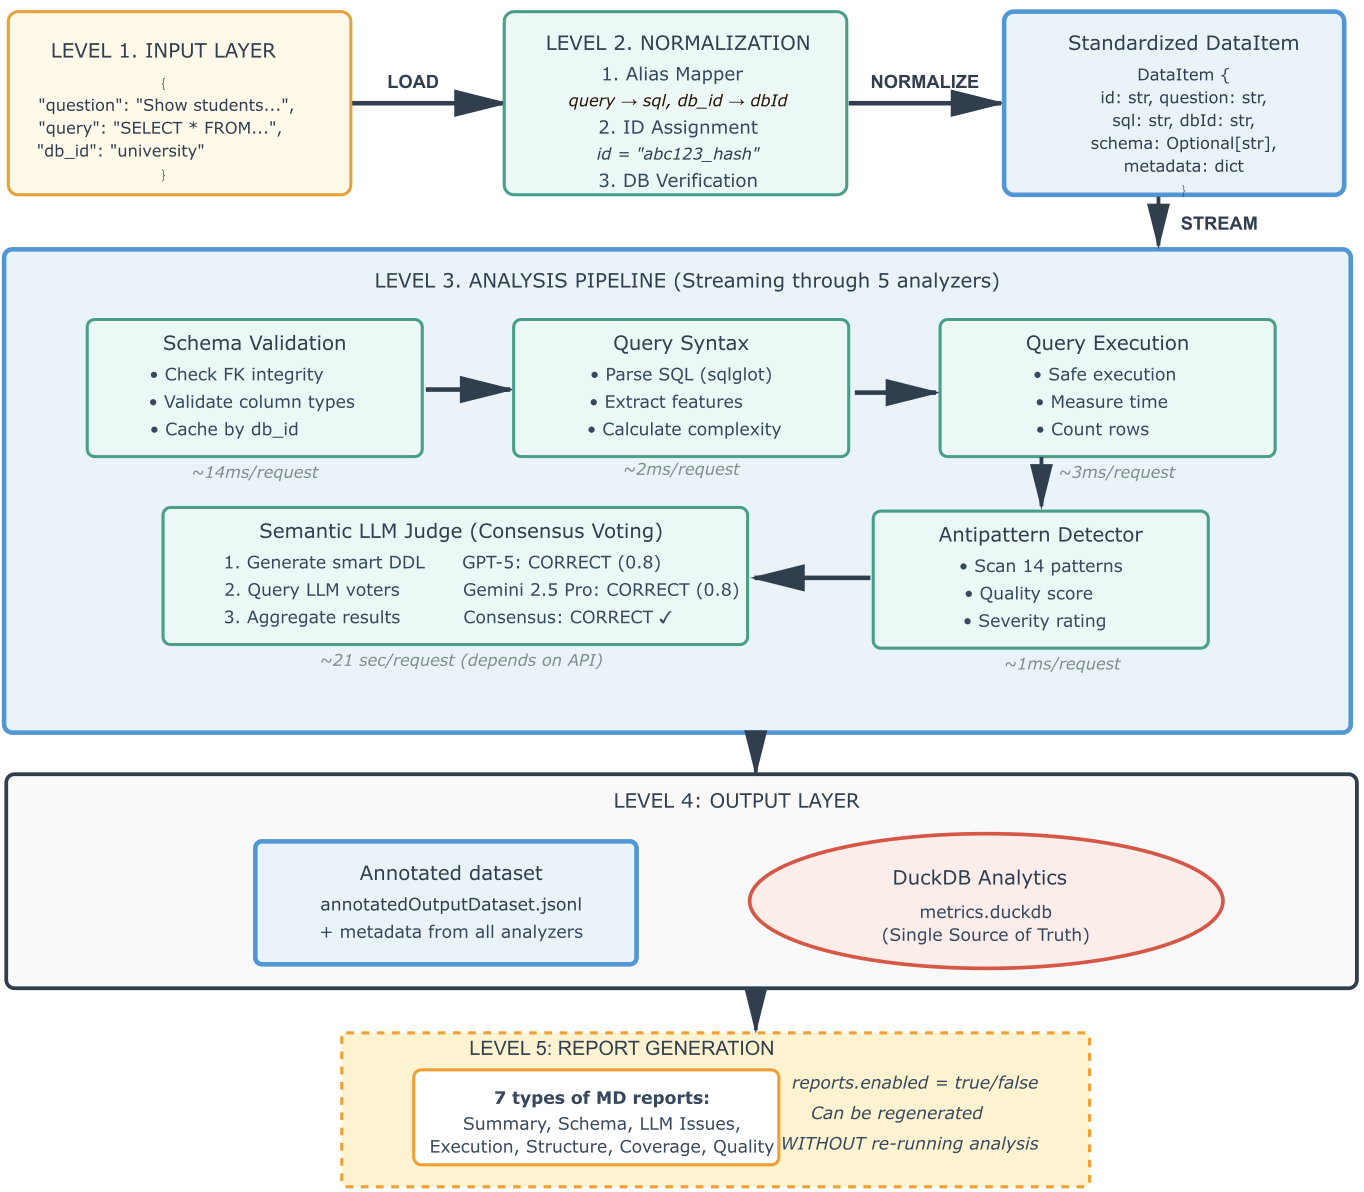
\includegraphics[width=0.85\textwidth]{figures/fig3_dataflow.png}
  \caption{Data flow through the pipeline from input to output}
  \label{fig:dataflow}
\end{figure}

The last report layer, which can be disabled via configuration (\texttt{reports.enabled = false}), reads metrics from DuckDB and produces seven types of human-readable analytical reports in Markdown format.

\subsection{Database Identity Normalization Algorithm}\label{sec:dbidentity}

The Database Identity Normalizer addresses a fundamental challenge in Text-to-SQL dataset processing: ensuring that every record can be associated with a valid, accessible database instance against which queries can be validated.

\begin{figure}[htbp]
  \centering
  
\includegraphics[width=0.75\textwidth]{figures/fig4_dbidentity.png}
  \caption{DbIdentity normalization process: guaranteed dbId filling via health check or creation from DDL}
  \label{fig:dbidentity}
\end{figure}

The algorithm implements a decision tree with three primary branches corresponding to different combinations of database identifier presence and schema availability (Figure~\ref{fig:dbidentity}).

In the first scenario, when a record provides an explicit database identifier, the normalizer invokes a health check through the database manager, querying whether the referenced database exists and contains data. If the check passes, the record proceeds unchanged; if it fails, the normalizer attempts to recreate the database from its stored DDL schema.

The second scenario handles records lacking explicit database identifiers but including DDL schema specifications, a pattern commonly encountered in synthetic datasets or benchmark subsets designed for isolated evaluation. The normalizer computes a deterministic hash of the DDL content to derive a unique database identifier, checks whether a database with that identifier already exists, and creates one if necessary.

The third scenario represents failure cases where records provide neither a database identifier nor a DDL schema. In this situation, the normalizer raises a \texttt{ValueError} with a descriptive error message, halting processing to prevent downstream analyzers from operating on incomplete data.

\subsection{Multi-Model Semantic Validation Architecture}\label{sec:semantic}

The Semantic LLM Judge Analyzer constitutes the most sophisticated component of our validation pipeline, employing large language models to assess whether SQL queries correctly answer their associated natural-language questions.

\textbf{Smart DDL Generation.} The first stage addresses the token efficiency challenge inherent in providing database schema context to language models. Naïvely transmitting complete database schemas can consume thousands of tokens per query, making large-scale validation prohibitively expensive.

\begin{figure}[htbp]
  \centering
  
\includegraphics[width=0.8\textwidth]{figures/fig5_semantic_judge.png}
  \caption{Architecture of the Semantic LLM Judge with multi-model consensus voting}
  \label{fig:semantic_judge}
\end{figure}

The smart DDL generator analyzes the SQL query's abstract syntax tree to identify all referenced tables and columns, retrieves schema metadata (column types, constraints) and sample data for those specific columns, and formats this information into minimal CREATE TABLE statements with inline comments containing example values.

\textbf{Prompt Template Resolution.} The second stage combines the generated smart DDL with contextual elements to produce complete evaluation prompts. Templates are loaded from YAML configuration files to facilitate experimentation with different prompt strategies. Key variables include:

\begin{itemize}
\item \texttt{\{\{question\}\}}: The natural language question from the dataset
\item \texttt{\{\{sql\}\}}: The SQL query under evaluation
\item \texttt{\{\{ddl\_schema\}\}}: The smart DDL from Stage 1
\item \texttt{\{\{dialect\}\}}: Optional SQL dialect specification (sqlite, postgresql, etc.)
\end{itemize}

The assembled prompt specifies a strictly structured response format in which the model must return a single JSON object with exactly two keys, ``verdict'' and ``explanation'' (Figure~\ref{fig:prompt_structure}). The ``verdict'' field must contain one of four enumerated values: CORRECT (query correctly and completely answers the question), PARTIALLY\_CORRECT (query answers part of the question or includes minor errors), INCORRECT (query does not answer the question or contains fundamental errors), or UNANSWERABLE (the question cannot be answered given the schema).

\begin{figure}[htbp]
  \centering
  
\includegraphics[width=0.85\textwidth]{figures/fig7_prompt.png}
  \caption{LLM prompt structure with input parameters, evaluation criteria, and four-category verdict classification}
  \label{fig:prompt_structure}
\end{figure}

The ``explanation'' field encodes a short natural-language justification; for CORRECT verdicts, the explanation is required to be an empty string, thereby preventing spurious narrative output, while for other verdicts it must describe the specific issue identified.

\textbf{Multi-Model Consensus Voting.} This stage queries multiple language models in parallel, collecting independent judgments. Our architecture supports four provider categories:

\begin{itemize}
\item \textbf{OpenAI models} (GPT-4o, GPT-4-turbo, etc.) provide strong reasoning capabilities and reliable structured output generation.
\item \textbf{Anthropic models} (Claude-3.5-sonnet, Claude-3-sonnet, etc.) offer alternative reasoning approaches that often exhibit different error patterns from GPT models.
\item \textbf{Google models} (Gemini-2.5-pro, Gemini-1.5-pro, etc.) deliver competitive performance with distinct training data and architectural choices.
\item \textbf{Ollama models} (Llama-3.1-70b, Mistral, Mixtral, etc.) enable fully local execution without API costs or rate limits.
\end{itemize}

Each model returns a structured response containing a verdict classification, a confidence score (0.0--1.0) indicating judgment certainty, and a free-text explanation articulating the reasoning.

\textbf{Consensus Decision.} The fourth stage aggregates the individual model responses through weighted voting to determine consensus verdicts and identify cases requiring human review. Each model is associated with a configurable weight reflecting its empirical reliability. The weighted consensus score is computed as:

\begin{equation}
\text{score}_{\text{consensus}} = \frac{\sum_{i=1}^{n} w_i \cdot v_i}{\sum_{i=1}^{n} w_i}
\end{equation}

where $v_i$ denotes the mapped verdict value and $w_i$ the corresponding model weight. This score captures the aggregate tendency of weighted models to regard a query as semantically adequate, while the majority verdict provides a discrete classification for reporting purposes.

The multi-model semantic validation architecture addresses several research challenges in Text-to-SQL evaluation. By employing multiple models with different architectures and training data, the system reduces single-model biases and provides uncertainty estimates through inter-model agreement metrics.

\subsection{Protocol-Based Architecture and Dependency Injection}

The system architecture employs Python's Protocol typing construct to establish clear contracts between components while maintaining loose coupling between interface definitions and their concrete implementations.

\begin{figure}[htbp]
  \centering
  
\includegraphics[width=0.8\textwidth]{figures/fig8_protocols.png}
  \caption{Protocol-based architecture with automatic dependency injection}
  \label{fig:protocols}
\end{figure}

This architectural pattern, analogous to interface-based programming in statically typed languages, provides the benefits of explicit type checking and interface documentation while preserving the flexibility and rapid iteration characteristics of dynamic Python development (Figure~\ref{fig:protocols}).

The \textbf{AnnotatingAnalyzer Protocol} defines the essential contract that all analyzer implementations must satisfy, specifying required attributes including a string-valued name identifier and a boolean enabled flag for runtime toggling.

The \textbf{MetricsSink Protocol} abstracts the mechanisms through which analyzers persist their computed metrics, defining three essential operations: write for accepting individual metric events, flush for ensuring durable persistence, and close for cleanup.

The \textbf{Normalizer Protocol} specifies the interface for components responsible for data standardization, requiring a normalize method that accepts an iterable of raw dictionary objects and returns an iterable of validated, enriched records.

The \textbf{DbAdapter Protocol} encapsulates dialect-specific database operations, defining methods for query execution with configurable safety modes, schema introspection for retrieving table and column metadata, and connection lifecycle management.

Component orchestration within the protocol-based architecture relies on the \texttt{dependency\_injector} library to automate the complex wiring of object graphs that arise from interdependent components. Each layer's components are registered in a declarative container specification, with dependencies expressed through type annotations.

The protocol-based architecture with dependency injection offers several significant advantages for research software development. The explicit protocol interfaces serve as machine-checkable documentation, automated dependency resolution eliminates manual wiring complexity, and the loose coupling between protocols and implementations facilitates testing through mock implementations.

\section{Experimental Setup and Results}\label{sec:Results}

\subsection{Experimental Methodology}

We select Spider 1.0 dataset as our primary test dataset because it has become the most widely used benchmark for both training and evaluating Text-to-SQL models in the research community. Its ubiquity means that quality issues in Spider propagate directly into hundreds of published studies and deployed systems.

The experimental methodology employs comprehensive multi-layer validation across all three Spider partitions (test, dev, train) to assess both overall dataset quality and consistency characteristics between training and evaluation subsets.

The three analyzed partitions exhibit substantially different scales: Spider Test contains 2,147 examples spanning 40 unique databases, Spider Dev includes 1,034 examples across 20 databases, and Spider Train encompasses 8,659 examples distributed over 146 databases.

All analyses employed SQLite as the target SQL dialect, matching Spider's native database format. The pipeline activated all five analyzers for all three partitions. The LLM configuration utilized Gemini-2.0-Flash-Exp and GPT-4o-mini with equal weights (0.5 each) for semantic validation, balancing accuracy and cost-effectiveness for large-scale evaluation.

Processing time varied substantially between partitions due to both dataset size and LLM API latency. Spider Test required approximately 12.7 hours when including LLM-based semantic validation, Spider Dev approximately 6.1 hours, and Spider Train approximately 50.3 hours.

\subsection{Database Schema Integrity Assessment}

Schema integrity validation examines the structural correctness of database definitions, detecting errors that could prevent successful query execution even for syntactically valid SQL statements. Table~\ref{tab:schema_overall} presents aggregate schema validation metrics across all three Spider partitions.

\begin{table}[ht]
    \caption{Comparative database schema validation results across Spider partitions}
    \label{tab:schema_overall}
    \centering
    \footnotesize
    \begin{tabular}{lcccc}
        \toprule
        \textbf{Metric} & \textbf{Spider Test} & \textbf{Spider Dev} & \textbf{Spider Train} & \textbf{Best} \\
        \midrule
        Total databases & 40 & 20 & 146 & -- \\
        Valid databases & 36 (90.0\%) & 13 (65.0\%) & 114 (78.1\%) & Test \\
        Invalid databases & 4 (10.0\%) & 7 (35.0\%) & 32 (21.9\%) & Test \\
        Total schema errors & 10 & 21 & 58 & Test \\
        Databases with FK violations & 4 & 7 & 27 & Test \\
        Total FK integrity violations & 0 & 2,400 & 38,273 & Test \\
        \bottomrule
    \end{tabular}
\end{table}

The results reveal a clear quality gradient across partitions, with Test achieving 90.0\% schema validity, substantially exceeding Train at 78.1\% and Dev at 65.0\%. This ordering contradicts the intuitive expectation that training data should exhibit higher quality than test data.

Analysis of error type distribution (Table~\ref{tab:schema_errors}) identifies dominant patterns contributing to schema invalidity. Foreign Key Type Mismatch errors, where referencing and referenced columns possess incompatible data types, constitute 39.1\% of all detected issues (34 of 89 total errors).

\begin{table}[ht]
    \caption{Distribution of schema error types across partitions}
    \label{tab:schema_errors}
    \centering
    \footnotesize
    \begin{tabular}{lccc}
        \toprule
        \textbf{Error Type} & \textbf{Spider Test} & \textbf{Spider Dev} & \textbf{Spider Train} \\
        \midrule
        Foreign Key Type Mismatch & 0 & 0 & 34 \\
        Foreign Key Target Not Found & 8 & 12 & 21 \\
        Duplicate Column Names & 2 & 9 & 3 \\
        \bottomrule
    \end{tabular}
\end{table}

A particularly concerning finding emerges from analysis of foreign key data integrity violations, distinct from the structural foreign key errors discussed above. While 10 databases across all partitions contain referential integrity violations, the distribution is highly skewed: sakila\_1 (Train) contains 38,273 violations and flight\_2 (Dev) contains 2,400 violations, together accounting for 99.5\% of all referential integrity problems.

The Train partition exhibits an additional quality issue absent from Test and Dev: 41 tables across 4 databases (academic, imdb, yelp, restaurants) contain schema definitions but no data rows, representing empty tables that cannot support meaningful query evaluation.

\subsection{Syntactic Structure and Complexity Analysis}

Syntactic analysis evaluates the structural characteristics of SQL queries independent of their semantic correctness, examining complexity, feature utilization, and parsing success rates. Table~\ref{tab:syntax_overall} demonstrates that Spider exhibits exceptional syntactic quality and strong cross-partition consistency.

\begin{table}[ht]
    \caption{Overall syntactic analysis results showing strong cross-partition consistency}
    \label{tab:syntax_overall}
    \centering
    \footnotesize
    \begin{tabular}{lcccc}
        \toprule
        \textbf{Metric} & \textbf{Spider Test} & \textbf{Spider Dev} & \textbf{Spider Train} & \textbf{Consistency} \\
        \midrule
        Total queries & 2,147 & 1,034 & 8,659 & -- \\
        Parsable queries & 2,147 (100\%) & 1,034 (100\%) & 8,659 (100\%) & Perfect \\
        Mean complexity & 28.3 & 28.7 & 29.1 & High \\
        Median complexity & 26.0 & 26.0 & 27.0 & High \\
        Complexity std.dev. & 13.2 & 13.5 & 14.1 & High \\
        \bottomrule
    \end{tabular}
\end{table}

The perfect parsing success rate (100\% across all 11,840 queries) constitutes a significant achievement, indicating that all queries conform to valid SQL syntax without requiring dialect-specific workarounds or manual corrections.

Examination of difficulty level distributions (Table~\ref{tab:difficulty}) reinforces this consistency pattern, with Easy/Medium/Hard categories exhibiting nearly identical proportions across Test and Dev partitions. Train shows slightly elevated complexity with a higher proportion of Hard queries (24.4\% vs 20.8\% in Test).

\begin{table}[ht]
    \caption{Query difficulty distribution across partitions}
    \label{tab:difficulty}
    \centering
    \footnotesize
    \begin{tabular}{lcccc}
        \toprule
        \textbf{Difficulty} & \textbf{Spider Test} & \textbf{Spider Dev} & \textbf{Spider Train} & \textbf{Range} \\
        \midrule
        Easy & 40.5\% & 39.8\% & 37.2\% & 3.3 pp \\
        Medium & 28.9\% & 30.7\% & 29.1\% & 1.8 pp \\
        Hard & 20.8\% & 20.6\% & 24.4\% & 3.8 pp \\
        Extra Hard & 9.8\% & 8.9\% & 8.5\% & 1.3 pp \\
        \bottomrule
    \end{tabular}
\end{table}

One notable exception to cross-partition consistency emerges in the Expert difficulty category: Train contains 66 Expert-level queries (0.8\% of the partition) while Test and Dev contain none. These 66 queries represent the most structurally complex examples in the entire Spider dataset.

Analysis of JOIN distribution (Table~\ref{tab:joins}) reveals a second dimension where Train exhibits systematically higher complexity compared to Test and Dev. Train contains a substantially larger proportion of multi-table queries involving 3+ JOINs (7.7\% vs 5.4\% in Test and 5.5\% in Dev).

\begin{table}[ht]
    \caption{JOIN distribution analysis showing Train's higher multi-table complexity}
    \label{tab:joins}
    \centering
    \footnotesize
    \begin{tabular}{lcccc}
        \toprule
        \textbf{JOIN Count} & \textbf{Spider Test} & \textbf{Spider Dev} & \textbf{Spider Train} & \textbf{Best} \\
        \midrule
        0 JOINs & 57.2\% & 55.1\% & 54.3\% & Test \\
        1 JOIN & 23.2\% & 24.3\% & 22.8\% & Dev \\
        2 JOINs & 14.2\% & 15.1\% & 15.2\% & Train \\
        3+ JOINs & 5.4\% & 5.5\% & 7.7\% & Train \\
        \bottomrule
    \end{tabular}
\end{table}

Despite the rich structural variation in JOIN complexity and overall difficulty levels, Spider exhibits complete absence of certain advanced SQL features. No queries in any partition employ common table expressions (WITH clauses), window functions (ROW\_NUMBER, RANK, LAG), or recursive queries.

\subsection{Dynamic Executability Validation}

Dynamic execution testing validates that syntactically correct queries can run against their associated databases, detecting semantic errors, missing tables/columns, type incompatibilities, and other runtime failures. Table~\ref{tab:execution} presents execution validation results.

\begin{table}[ht]
    \caption{Query execution results showing exceptional executability rates}
    \label{tab:execution}
    \centering
    \footnotesize
    \begin{tabular}{lcccc}
        \toprule
        \textbf{Metric} & \textbf{Spider Test} & \textbf{Spider Dev} & \textbf{Spider Train} & \textbf{Best} \\
        \midrule
        Total queries & 2,147 & 1,034 & 8,659 & -- \\
        Executable queries & 2,147 (100\%) & 1,034 (100\%) & 8,656 (99.97\%) & Test/Dev \\
        Failed executions & 0 (0\%) & 0 (0\%) & 3 (0.03\%) & Test/Dev \\
        Mean execution time (ms) & 3.10 & 2.49 & 1.19 & Train \\
        \bottomrule
    \end{tabular}
\end{table}

The execution success rates—100\% for Test and Dev, 99.97\% for Train—represent a remarkable achievement given the complexity of the queries and the schema integrity issues documented in Section~\ref{sec:Results}. The three failed queries in Train all stem from references to non-existent columns resulting from schema definition errors.

\subsection{Code Quality Assessment via Antipattern Detection}

Antipattern detection identifies common SQL coding practices that, while syntactically valid and functionally correct, deviate from established best practices regarding performance, maintainability, or security. Table~\ref{tab:antipatterns_overall} summarizes code quality metrics.

\begin{table}[ht]
    \caption{Overall code quality metrics showing consistent high quality}
    \label{tab:antipatterns_overall}
    \centering
    \footnotesize
    \begin{tabular}{lcccc}
        \toprule
        \textbf{Metric} & \textbf{Spider Test} & \textbf{Spider Dev} & \textbf{Spider Train} & \textbf{Best} \\
        \midrule
        Queries with 0 antipatterns & 15.4\% & 14.8\% & 15.2\% & Test \\
        Mean antipatterns per query & 1.02 & 1.04 & 1.03 & Test \\
        Median antipatterns per query & 1.0 & 1.0 & 1.0 & All equal \\
        \bottomrule
    \end{tabular}
\end{table}

Most detected antipatterns are stylistic (SELECT *, missing LIMIT) rather than logical errors, do not affect query execution correctness or result accuracy, and represent acceptable trade-offs in dataset design priorities.

Table~\ref{tab:antipatterns_top5} confirms this hypothesis, revealing that Unbounded SELECT (queries lacking LIMIT clauses) dominates the antipattern distribution. In Test, 84.6\% of queries lack LIMIT clauses, explaining why the mean antipatterns per query remains close to 1.0.

\begin{table}[ht]
    \caption{Top-5 most frequent antipatterns}
    \label{tab:antipatterns_top5}
    \centering
    \footnotesize
    \begin{tabular}{lcccc}
        \toprule
        \textbf{Antipattern} & \textbf{Spider Test} & \textbf{Spider Dev} & \textbf{Spider Train} & \textbf{Severity} \\
        \midrule
        Unbounded SELECT & 84.6\% & 85.3\% & 85.1\% & Low \\
        SELECT * & 5.2\% & 4.8\% & 5.1\% & Low \\
        Function in WHERE & 3.1\% & 3.4\% & 2.9\% & Medium \\
        Correlated subquery & 2.8\% & 2.6\% & 2.7\% & Medium \\
        \bottomrule
    \end{tabular}
\end{table}

\subsection{Semantic Correctness via LLM Consensus}

Semantic validation represents the most critical quality dimension, as syntactically valid, successfully executing queries may nonetheless fail to correctly answer their associated natural language questions. Table~\ref{tab:semantic} presents consensus verdicts from two-model LLM validation (Gemini-2.0-Flash-Exp and GPT-4o-mini with equal weights).

\begin{table}[ht]
    \caption{Semantic validation results via LLM consensus voting}
    \label{tab:semantic}
    \centering
    \footnotesize
    \begin{tabular}{lccc}
        \toprule
        \textbf{Consensus Verdict} & \textbf{Spider Test} & \textbf{Spider Dev} & \textbf{Spider Train} \\
        \midrule
        CORRECT & 70.4\% & 64.5\% & 60.0\% \\
        PARTIALLY\_CORRECT & 7.3\% & 7.8\% & 9.2\% \\
        INCORRECT & 2.6\% & 1.6\% & 3.5\% \\
        UNANSWERABLE & 1.2\% & 1.2\% & 1.3\% \\
        MIXED (disagreement) & 18.5\% & 24.9\% & 26.0\% \\
        \bottomrule
    \end{tabular}
\end{table}

The Mixed verdict category, indicating model disagreement, warrants particular attention given its substantial prevalence across all partitions. Train exhibits the highest Mixed rate (26.0\%), followed by Dev (24.9\%) and Test (18.5\%), suggesting that larger partitions contain more ambiguous or underspecified examples where reasonable SQL implementations could differ.

Table~\ref{tab:semantic_categories} synthesizes these findings into actionable quality categories across all three partitions. High-confidence correct examples decline from 70.4\% in Test through 64.5\% in Dev to 60.0\% in Train, reinforcing the quality gradient observed in schema validation results.

\begin{table}[ht]
    \caption{Semantic quality categorization summary}
    \label{tab:semantic_categories}
    \centering
    \footnotesize
    \begin{tabular}{lccc}
        \toprule
        \textbf{Category} & \textbf{Spider Test} & \textbf{Spider Dev} & \textbf{Spider Train} \\
        \midrule
        High-confidence correct & 70.4\% & 64.5\% & 60.0\% \\
        Possibly correct (mixed) & 18.5\% & 24.9\% & 26.0\% \\
        Needs review (partial/incorrect) & 9.9\% & 9.4\% & 12.7\% \\
        Unanswerable & 1.2\% & 1.2\% & 1.3\% \\
        \bottomrule
    \end{tabular}
\end{table}

\subsection{Integrated Quality Assessment and Recommendations}

The comprehensive multi-layer analysis of Spider's three partitions enables an integrated quality assessment synthesizing findings across all validation dimensions. Table~\ref{tab:integrated} summarizes key quality indicators.

\begin{table}[ht]
    \caption{Integrated quality assessment across all validation dimensions}
    \label{tab:integrated}
    \centering
    \footnotesize
    \begin{tabular}{lcccc}
        \toprule
        \textbf{Quality Criterion} & \textbf{Test} & \textbf{Dev} & \textbf{Train} & \textbf{Best} \\
        \midrule
        Schema validity & 90.0\% & 65.0\% & 78.1\% & Test \\
        SQL parsability & 100\% & 100\% & 100\% & All \\
        SQL executability & 100\% & 100\% & 99.97\% & Test/Dev \\
        Semantic correctness & 70.4\% & 64.5\% & 60.0\% & Test \\
        Low antipattern rate & 15.4\% & 14.8\% & 15.2\% & Test \\
        \bottomrule
    \end{tabular}
\end{table}

The analysis identifies both strengths and critical weaknesses in Spider's construction. On the positive side, the dataset achieves exceptional syntactic quality with 100\% parsing success across all 11,840 queries and near-perfect executability (99.97\%+), demonstrating careful query construction and thorough validation of SQL correctness.

The most severe problem identified concerns referential integrity violations concentrated in two databases: sakila\_1 (Train) with 38,273 violations and flight\_2 (Dev) with 2,400 violations. Together these represent 40,673 referential integrity errors affecting approximately 485 queries (5.6\% of Train and 23.3\% of Dev).

Based on these findings, we propose a prioritized remediation roadmap:

\textbf{Critical priority actions}: immediate investigation and repair of sakila\_1 and flight\_2 databases to eliminate the 40,673 referential integrity violations; manual review of the 1,164 queries (9.8\% of dataset) flagged as PARTIALLY\_CORRECT or INCORRECT by LLM consensus to identify and correct semantic misalignments.

\textbf{Recommended improvements}: systematic correction of the 34 Foreign Key Type Mismatch errors in Train through database schema modifications; resolution of the 41 Foreign Key Target Not Found errors across all partitions by adding missing indexes or removing invalid foreign key constraints.

\textbf{Optional enhancements}: adding LIMIT clauses to unbounded SELECT queries where semantically appropriate; replacing SELECT * with explicit column lists in the 5\% of queries exhibiting this antipattern.

\section{Discussion}\label{sec:Discussion}

\subsection{Summary of Findings}

Our analysis shows that Spider is syntactically robust and almost perfectly executable, but it is not free of technical and semantic issues. Structural schema problems, especially in a subset of databases with referential integrity violations, affect a non-trivial proportion of training and evaluation examples. Semantic validation using LLMs reveals that 30--40\% of queries receive non-CORRECT verdicts or exhibit inter-model disagreement, suggesting potential ambiguities or misalignments invisible to execution-based metrics.

\subsection{Implications for Benchmark Use}

For researchers, these findings imply that benchmark scores on Spider should be interpreted with caution. Models might achieve high execution accuracy while being trained and evaluated on data that contains semantic inconsistencies or structural defects, leading to overfitting to dataset artifacts rather than generalizable Text-to-SQL capabilities.

For dataset maintainers, the identified issues provide a concrete prioritized roadmap. Addressing the two databases responsible for many referential integrity violations would substantially improve structural quality with minimal effort, while systematic review of queries flagged by LLM judges could reduce semantic ambiguities.

\subsection{Threats to Validity}

The primary threat to validity in our study is that semantic validation relies on only two large language models as judges. Although we deliberately select models from different providers and require consensus for high-confidence verdicts, both models could share systematic biases or misconceptions about SQL semantics. Future work should expand the judge panel to include additional model families and incorporate human expert validation for a statistically significant sample.

A second threat is the limited scope of human verification. Manual inspection was performed only for the Unanswerable category, which constitutes a small fraction of all examples. While this focus is justified given resource constraints, comprehensive human review of all MIXED and INCORRECT cases would strengthen confidence in semantic validity conclusions.

\section{Conclusions and Future Work}\label{sec:Conclusions}

We presented \texttt{text2sql-pipeline}, the first open-source framework for comprehensive Text-to-SQL dataset validation and applied it to a full-scale audit of the Spider 1.0 benchmark. The framework integrates five complementary quality dimensions—schema integrity, syntactic correctness, executability, code quality, and semantic alignment—into a unified streaming architecture supporting datasets of arbitrary scale.

Our empirical study of all three Spider partitions shows that, although the benchmark is syntactically well-formed and almost perfectly executable, it contains non-trivial structural defects and a significant proportion of semantically ambiguous or potentially incorrect examples. Specifically: 10--35\% of databases exhibit schema validity issues; 40,673 referential integrity violations are concentrated in just two databases; and 30--40\% of queries receive non-CORRECT or MIXED semantic verdicts from LLM judges.

These findings demonstrate that standard evaluation metrics (exact-match accuracy, execution-based metrics) are necessary but insufficient for assessing Text-to-SQL system quality. Multi-layer validation exposes latent quality issues that can influence model training dynamics and evaluation reliability.

Future work will extend the framework in several directions. First, we plan to add automatic repair suggestions for selected classes of problems, such as foreign key mismatches or simple semantic discrepancies. Second, we will conduct large-scale human annotation studies to establish ground truth for semantic correctness, enabling calibration of LLM judge reliability. Third, we will apply the framework to other major Text-to-SQL benchmarks (BIRD, CHASE, WikiSQL) to assess whether the quality patterns observed in Spider generalize to other datasets.

We hope that making dataset validation tools widely available will encourage the community to treat benchmark quality as a first-class research concern, ultimately leading to more reliable Text-to-SQL systems and more trustworthy empirical conclusions.

\subsection*{Acknowledgment}

The authors gratefully acknowledge the financial support of Intellias, which enabled the use of frontier large language models in this work.

\Funding{This research did not receive any specific grant from funding agencies in the public, commercial or not-for-profit sectors. The use of commercial LLM APIs was supported by Intellias.}

\Data{The developed Text-to-SQL analysis tool is available as open-source software on GitHub at https://github.com/vsabadosh/text2sql-dataset-analyzer. The repository contains all configuration files, scripts, and documentation required to reproduce the analyses presented in this paper.}

\CompetingInterests{The author declares that there are no known competing financial interests or personal relationships that could have appeared to influence the work reported in this paper.}

\Credits{
Volodymyr Sabadosh: Conceptualization, Software Design, Data curation, Formal analysis, Methodology, Investigation, Visualization, Writing -- original draft, Writing -- review and editing.
% See https://credit.niso.org/
}

\setbiblabelwidth{1000}
\bibliographystyle{IEEEtran_for_EI} 
\bibliography{text2sql_quality_paper}

\appendix
\makeatletter
\def\mw@seccntformat#1{Appendix\ #1.\enspace}
\makeatother

\section{Declaration of Generative AI Use}\label{sec:ai_declaration}

During the preparation of this work, the author used ChatGPT (OpenAI) and Claude (Anthropic) to improve the grammar, clarity and structure of the manuscript. After using these tools, the author carefully checked and edited the content as needed and takes full responsibility for the content of the publication.

\end{document}

